%%*****************************************************************************
%% $Id: bst-language.tex,v 0.00 2008/04/30 23:26:21 gene Exp $
%%*****************************************************************************
%% Author: Gerd Neugebauer
%%-----------------------------------------------------------------------------

\chapter{The BST Language}

\IM{08x1}%
The processing of the data base entries can be programmed with a small
special purpose programming language. Since it seems to habe no name
it is called the BST language

Usually the instructions are read from a file. The default extension
of these files is \texttt{.bst}. The content is interpreted to produce
the formatted output.

The primary goal of \BibTeX\ is the processing of bibliographic
databases. Thus the language is tailored towards the formatting of
bibliographies.

\section{The Programming Model}

The BST language is based on a simple stack based metaphor. The stack
is the central data structure in the program. The stack is able to
carry arbitrary data. Especially it is possible to push code segments
to the stack.

\begin{figure}[tb]
  \centering
  %%*****************************************************************************
%% Copyright (c) 2008 Gerd Neugebauer
%%
%% Permission is granted to copy, distribute and/or modify this document
%% under the terms of the GNU Free Documentation License, Version 1.2
%% or any later version published by the Free Software Foundation;
%% with no Invariant Sections, no Front-Cover Texts, and no Back-Cover Texts.
%%
%%*****************************************************************************
%% $Id:bst-model.tex 7067 2008-05-18 11:06:56Z gene $
%%*****************************************************************************
%% Author: Gerd Neugebauer
%%-----------------------------------------------------------------------------
\begingroup
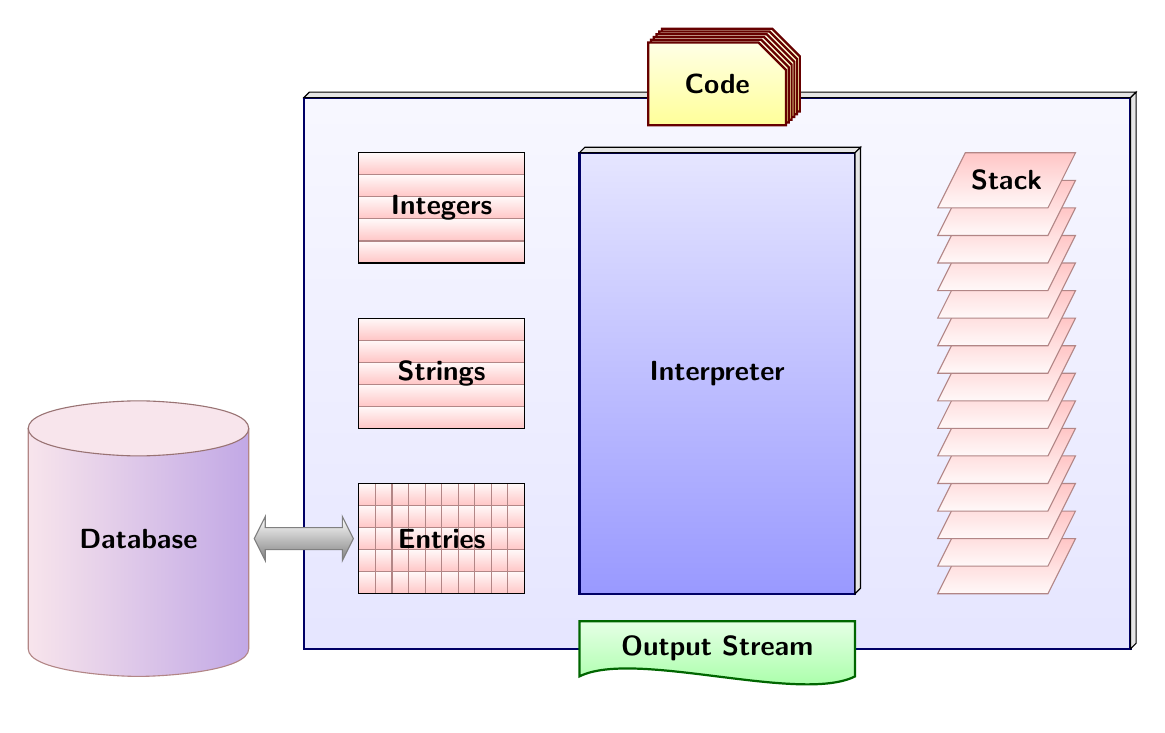
\begin{tikzpicture}[scale=.7]\sf\bfseries
  % --- bottom layer ---
  \shade[top color=white!97!blue,bottom color=white!90!blue,draw=blue!40!black,thick]
  (0,0) rectangle (15,10);
  \draw[fill=gray!20!white] (0,10) -- (.1,10.1) -- (15.1,10.1) -- (15,10) -- cycle;
  \draw[fill=gray!20!white] (15,10) -- (15.1,10.1) -- (15.1,.1) -- (15,0) -- cycle;

  % --- code ---
  \begin{scope}[shift={(6.25,9.5)},scale=.5]
    \begin{scope}[shift={(.5,.5)}]
      \shade[top color=white!90!yellow,bottom color=white!60!yellow,draw=red!40!black,thick]
      (0,0) -- (5,0) -- (5,2) -- (4,3) -- (0,3) -- cycle;
    \end{scope}
    \begin{scope}[shift={(.4,.4)}]
      \shade[top color=white!90!yellow,bottom color=white!60!yellow,draw=red!40!black,thick]
      (0,0) -- (5,0) -- (5,2) -- (4,3) -- (0,3) -- cycle;
    \end{scope}
    \begin{scope}[shift={(.3,.3)}]
      \shade[top color=white!90!yellow,bottom color=white!60!yellow,draw=red!40!black,thick]
      (0,0) -- (5,0) -- (5,2) -- (4,3) -- (0,3) -- cycle;
    \end{scope}
    \begin{scope}[shift={(.2,.2)}]
      \shade[top color=white!90!yellow,bottom color=white!60!yellow,draw=red!40!black,thick]
      (0,0) -- (5,0) -- (5,2) -- (4,3) -- (0,3) -- cycle;
    \end{scope}
    \begin{scope}[shift={(.1,.1)}]
      \shade[top color=white!90!yellow,bottom color=white!60!yellow,draw=red!40!black,thick]
      (0,0) -- (5,0) -- (5,2) -- (4,3) -- (0,3) -- cycle;
    \end{scope}
    \shade[top color=white!90!yellow,bottom color=white!60!yellow,draw=red!40!black,thick]
    (0,0) -- (5,0) -- (5,2) -- (4,3) -- (0,3) -- cycle;
  \end{scope}
  \draw (7.5,10.25) node {Code};

  % --- interpreter ---
  \shade[top color=white!90!blue,bottom color=white!60!blue,draw=blue!40!black,thick]
  (5,1) rectangle (10,9);
  \draw[fill=gray!20!white] (5,9) -- (5.1,9.1) -- (10.1,9.1) -- (10,9) -- cycle;
  \draw[fill=gray!20!white] (10,9) -- (10.1,9.1) -- (10.1,1.1) -- (10,1) -- cycle;
  \draw (7.5,5) node {Interpreter};
  
  \shade[top color=white!90!green,bottom color=white!60!green,draw=green!40!black,thick]
  (5,-.5) .. controls (6,0) and (9,-1) .. (10,-.5) -- (10,.5) -- (5,.5) -- cycle;
  \draw (7.5,0) node {Output Stream};


  % --- stack ---
  \shade[top color=white!10!pink,bottom color=white!90!pink,draw=pink!70!black,shift={(11.5,1)}] (0,0) -- (.5,1) -- (2.5,1) -- (2,0) -- cycle;
  \shade[top color=white!10!pink,bottom color=white!90!pink,draw=pink!70!black,shift={(11.5,1.5)}] (0,0) -- (.5,1) -- (2.5,1) -- (2,0) -- cycle;
  \shade[top color=white!10!pink,bottom color=white!90!pink,draw=pink!70!black,shift={(11.5,2)}] (0,0) -- (.5,1) -- (2.5,1) -- (2,0) -- cycle;
  \shade[top color=white!10!pink,bottom color=white!90!pink,draw=pink!70!black,shift={(11.5,2.5)}] (0,0) -- (.5,1) -- (2.5,1) -- (2,0) -- cycle;
  \shade[top color=white!10!pink,bottom color=white!90!pink,draw=pink!70!black,shift={(11.5,3)}] (0,0) -- (.5,1) -- (2.5,1) -- (2,0) -- cycle;
  \shade[top color=white!10!pink,bottom color=white!90!pink,draw=pink!70!black,shift={(11.5,3.5)}] (0,0) -- (.5,1) -- (2.5,1) -- (2,0) -- cycle;
  \shade[top color=white!10!pink,bottom color=white!90!pink,draw=pink!70!black,shift={(11.5,4)}] (0,0) -- (.5,1) -- (2.5,1) -- (2,0) -- cycle;
  \shade[top color=white!10!pink,bottom color=white!90!pink,draw=pink!70!black,shift={(11.5,4.5)}] (0,0) -- (.5,1) -- (2.5,1) -- (2,0) -- cycle;
  \shade[top color=white!10!pink,bottom color=white!90!pink,draw=pink!70!black,shift={(11.5,5)}] (0,0) -- (.5,1) -- (2.5,1) -- (2,0) -- cycle;
  \shade[top color=white!10!pink,bottom color=white!90!pink,draw=pink!70!black,shift={(11.5,5.5)}] (0,0) -- (.5,1) -- (2.5,1) -- (2,0) -- cycle;
  \shade[top color=white!10!pink,bottom color=white!90!pink,draw=pink!70!black,shift={(11.5,6)}] (0,0) -- (.5,1) -- (2.5,1) -- (2,0) -- cycle;
  \shade[top color=white!10!pink,bottom color=white!90!pink,draw=pink!70!black,shift={(11.5,6.5)}] (0,0) -- (.5,1) -- (2.5,1) -- (2,0) -- cycle;
  \shade[top color=white!10!pink,bottom color=white!90!pink,draw=pink!70!black,shift={(11.5,7)}] (0,0) -- (.5,1) -- (2.5,1) -- (2,0) -- cycle;
  \shade[top color=white!10!pink,bottom color=white!90!pink,draw=pink!70!black,shift={(11.5,7.5)}] (0,0) -- (.5,1) -- (2.5,1) -- (2,0) -- cycle;
  \shade[top color=white!10!pink,bottom color=white!90!pink,draw=pink!70!black,shift={(11.5,8)}] (0,0) -- (.5,1) -- (2.5,1) -- (2,0) -- cycle;
  \draw (12.75,8.5) node {Stack};

  % --- integers ---
  \shade[top color=white!90!pink,bottom color=white!10!pink,draw=pink!70!black]
  (1,7) rectangle (4,7.4);
  \shade[shift={(0,.4)},top color=white!90!pink,bottom color=white!10!pink,draw=pink!70!black]
  (1,7) rectangle (4,7.4);
  \shade[shift={(0,.8)},top color=white!90!pink,bottom color=white!10!pink,draw=pink!70!black]
  (1,7) rectangle (4,7.4);
  \shade[shift={(0,1.2)},top color=white!90!pink,bottom color=white!10!pink,draw=pink!70!black]
  (1,7) rectangle (4,7.4);
  \shade[shift={(0,1.6)},top color=white!90!pink,bottom color=white!10!pink,draw=pink!70!black]
  (1,7) rectangle (4,7.4);
  \draw (1,7) rectangle (4,9);
  \draw (2.5,8) node {Integers};

  % --- strings ---
  \shade[top color=white!90!pink,bottom color=white!10!pink,draw=pink!70!black]
  (1,4) rectangle (4,4.4);
  \shade[shift={(0,.4)},top color=white!90!pink,bottom color=white!10!pink,draw=pink!70!black]
  (1,4) rectangle (4,4.4);
  \shade[shift={(0,.8)},top color=white!90!pink,bottom color=white!10!pink,draw=pink!70!black]
  (1,4) rectangle (4,4.4);
  \shade[shift={(0,1.2)},top color=white!90!pink,bottom color=white!10!pink,draw=pink!70!black]
  (1,4) rectangle (4,4.4);
  \shade[shift={(0,1.6)},top color=white!90!pink,bottom color=white!10!pink,draw=pink!70!black]
  (1,4) rectangle (4,4.4);
  \draw (1,4) rectangle (4,6);
  \draw (2.5,5) node {Strings};

  % --- entries ---
  \shade[top color=white!90!pink,bottom color=white!10!pink,draw=pink!70!black]
  (1,1) rectangle (4,1.4);
  \shade[shift={(0,.4)},top color=white!90!pink,bottom color=white!10!pink,draw=pink!70!black]
  (1,1) rectangle (4,1.4);
  \shade[shift={(0,.8)},top color=white!90!pink,bottom color=white!10!pink,draw=pink!70!black]
  (1,1) rectangle (4,1.4);
  \shade[shift={(0,1.2)},top color=white!90!pink,bottom color=white!10!pink,draw=pink!70!black]
  (1,1) rectangle (4,1.4);
  \shade[shift={(0,1.6)},top color=white!90!pink,bottom color=white!10!pink,draw=pink!70!black]
  (1,1) rectangle (4,1.4);
  \draw[shift={(.3,0)},draw=pink!70!black] (1,1) -- (1,3);
  \draw[shift={(.6,0)},draw=pink!70!black] (1,1) -- (1,3);
  \draw[shift={(.9,0)},draw=pink!70!black] (1,1) -- (1,3);
  \draw[shift={(1.2,0)},draw=pink!70!black] (1,1) -- (1,3);
  \draw[shift={(1.5,0)},draw=pink!70!black] (1,1) -- (1,3);
  \draw[shift={(1.8,0)},draw=pink!70!black] (1,1) -- (1,3);
  \draw[shift={(2.1,0)},draw=pink!70!black] (1,1) -- (1,3);
  \draw[shift={(2.4,0)},draw=pink!70!black] (1,1) -- (1,3);
  \draw[shift={(2.7,0)},draw=pink!70!black] (1,1) -- (1,3);
  \draw (1,1) rectangle (4,3);
  \draw (2.5,2) node {Entries};

  \begin{scope}[shift={(-5,0)}]
    \shade[left color=white!96!blue!70!pink,right color=white!60!blue!60!pink,draw=pink!70!black]
    (0,0)   .. controls (0,-.4) and (1.5,-.5) ..
    (2,-.5)  .. controls (2.5,-.5) and (4,-.4) ..
    (4,0) -- (4,4) -- (0,4) -- cycle;
    \draw[shift={(0,4)},fill=white!96!blue!70!pink,draw=pink!60!black]
    (0,0)   .. controls (0,.4) and (1.5,.5) ..
    (2,.5)  .. controls (2.5,.5) and (4,.4) ..
    (4,0)   .. controls (4,-.4) and (2.5,-.5) ..
    (2,-.5) .. controls (1.5,-.5) and (0,-.4) ..
    (0,0);
  \end{scope}
  \draw (-3,2) node {Database};

%  \draw[shift={(0,-5)}]
%  (-.2,0) -- (0,.4) -- (0,.2) -- (1,.2) -- (1,.4) -- (1.2,0) --
%  (1,-.4) -- (1,-.2) -- (0,-.2) -- (0,-.4) -- cycle;

  \shade[shift={(-.7,2)}, top color=white, bottom color=gray,draw=gray]
  (-.2,0) -- (0,.4) -- (0,.2) -- (1.4,.2) -- (1.4,.4) -- (1.6,0) --
  (1.4,-.4) -- (1.4,-.2) -- (0,-.2) -- (0,-.4) -- cycle;

\end{tikzpicture}
\endgroup
\endinput
%
% Local Variables: 
% mode: latex
% TeX-master: nil
% End: 

  \caption{The BST Programming Model}
  \label{fig:bst-model}
\end{figure}


\subsection{The Database Context}

Whenever a bst program is executed a database is at hand. The porogram
has access to this database.

\INCOMPLETE

\subsection{Global Integers}

\INCOMPLETE

\subsection{Global Strings}

\INCOMPLETE

\subsection{Code}

\INCOMPLETE


\section{Syntax}

\INCOMPLETE

\section{Commands}


\subsection{\texttt{entry}}

\INCOMPLETE

\subsection{\texttt{integers}}

\INCOMPLETE

\begin{lstlisting}{}
  INTEGERS { output.state before.all }
\end{lstlisting}

\subsection{\texttt{strings}}

\INCOMPLETE

\begin{lstlisting}{}
  STRINGS { s t }
\end{lstlisting}

\subsection{\texttt{macro}}

\INCOMPLETE

\begin{lstlisting}{}
  MACRO {jan} {"January"}
\end{lstlisting}

\subsection{\texttt{execute}}

\INCOMPLETE

\begin{lstlisting}{}
  EXECUTE {begin.bib}
\end{lstlisting}

\subsection{\texttt{iterate}}

\INCOMPLETE

\begin{lstlisting}{}
  ITERATE{call.type$}
\end{lstlisting}

\subsection{\texttt{reverse}}

\INCOMPLETE

\begin{lstlisting}{}
  REVERSE{reverse.pass}
\end{lstlisting}

\subsection{\texttt{sort}}

\INCOMPLETE

\begin{lstlisting}{}
  SORT
\end{lstlisting}

\subsection{\texttt{read}}

\INCOMPLETE

\begin{lstlisting}{}
  READ
\end{lstlisting}

\subsection{\texttt{function}}

\INCOMPLETE

\begin{lstlisting}{}
  FUNCTION {sortify}
  { purify$
    "l" change.case$
  }
\end{lstlisting}


\subsection{\texttt{input}}
\IM{x}

\INCOMPLETE

\begin{lstlisting}{}
  INPUT{some/other/bst}
\end{lstlisting}

\section{Instructions}

\subsection{\texttt{>}}

\INCOMPLETE

\subsection{\texttt{<}}

\INCOMPLETE

\subsection{\texttt{=}}

\INCOMPLETE

\subsection{\texttt{+}}

\INCOMPLETE

\subsection{\texttt{-}}

\INCOMPLETE

\subsection{\texttt{*}}

\INCOMPLETE

\subsection{\texttt{:=}}

\INCOMPLETE

\subsection{\texttt{add.period\$}}

\INCOMPLETE

\subsection{\texttt{call.type\$}}

\INCOMPLETE

\subsection{\texttt{change.case\$}}

\INCOMPLETE

\subsection{\texttt{chr.to.int\$}}

\INCOMPLETE

\subsection{\texttt{cite\$}}

\begin{lstlisting}{}
  cite$
\end{lstlisting}

\INCOMPLETE

\subsection{\texttt{duplicate\$}}

\INCOMPLETE

\subsection{\texttt{empty\$}}

\INCOMPLETE

\subsection{\texttt{format.name\$}}

\INCOMPLETE

\subsection{\texttt{if\$}}

\INCOMPLETE

\subsection{\texttt{int.to.chr\$}}

\INCOMPLETE

\subsection{\texttt{int.to.str\$}}

\INCOMPLETE

\subsection{\texttt{missing\$}}

\INCOMPLETE

\subsection{\texttt{newline\$}}

This instruction writes a newline character to the output stream.

\begin{lstlisting}{}
  newline$
\end{lstlisting}

\subsection{\texttt{num.names\$}}

\INCOMPLETE

\subsection{\texttt{pop\$}}

\INCOMPLETE

\subsection{\texttt{preamble\$}}

\INCOMPLETE

\subsection{\texttt{purify\$}}

\INCOMPLETE

\subsection{\texttt{quote\$}}

\INCOMPLETE

\subsection{\texttt{skip\$}}

This instruction does simply nothing. In other languages this might be
called a noop. This is useful for places where instructions are
mandatory but nothing should be done.

\subsection{\texttt{stack\$}}

\INCOMPLETE

\subsection{\texttt{substring\$}}

\INCOMPLETE

\subsection{\texttt{swap\$}}

This instruction takes the two topmost elements from the stack and
exchanges their order on the stack. This means that the topmost
element becomes the second one and the second element becomes the
topmost one. The elements can be of any type.

If there are less than two elements on the stack then an error is
raised.

\subsection{\texttt{text.length\$}}

\INCOMPLETE

\subsection{\texttt{text.prefix\$}}

\INCOMPLETE

\subsection{\texttt{top\$}}

\INCOMPLETE

\subsection{\texttt{type\$}}

\INCOMPLETE

\subsection{\texttt{warning\$}}

This instruction pops a string from the stack and prints it as a
warning to the log stream.

\subsection{\texttt{while\$}}

\INCOMPLETE

\subsection{\texttt{width\$}}

This instruction pops a string from the stack and tries to compute the
width of the string when tyoeset. For this purpose the width of the
characters in the font cmr10 are used.

\subsection{\texttt{write\$}}

This instruction pops a string from the stack and prints it as a
message to the output stream.


\endinput
%
% Local Variables: 
% mode: latex
% TeX-master: "exbib-users"
% End: 
